\documentclass[10pt,xcolor=pdflatex]{beamer}
\usepackage{newcent}
\usepackage[utf8]{inputenc}
\usepackage[czech]{babel}
\usepackage{hyperref}
\usepackage{fancyvrb}
\usepackage{graphicx}
\usepackage{textpos}
\usepackage{tikz}
\usepackage{textcomp}
\usepackage[export]{adjustbox}
\usepackage{float}
\usepackage{alltt}
\usepackage{hyperref}
\usepackage{textpos}
\usepackage{multicol}
\usepackage{tikz}
\usepackage{fancyvrb}
\usepackage{color}
\usepackage{subfig}
\usepackage{geometry}
\usepackage{graphicx}
\usepackage{epstopdf}
\usepackage{multicol}
\usetheme{FIT}

\newcommand{\myuv}[1]{\quotedblbase #1\textquotedblleft}
\def\uv#1{\quotedblbase#1\textquotedblleft}%

%%%%%%%%%%%%%%%%%%%%%%%%%%%%%%%%%%%%%%%%%%%%%%%%%%%%%%%%%%%%%%%%%%
\title[GJA 2]{Testing, Maven and JAX}

\author[]{Jaroslav Dytrych}

\institute[]{Faculty of Information Technology
Brno University of Technology \\
Bo\v{z}et\v{e}chova 1/2. 612 66 Brno - Kr\'alovo Pole\\
dytrych@fit.vutbr.cz}

\date{26 September 2023}
%\date{\today}
%\date{} % bez data

%%%%%%%%%%%%%%%%%%%%%%%%%%%%%%%%%%%%%%%%%%%%%%%%%%%%%%%%%%%%%%%%%%

\begin{document}

\frame[plain]{\titlepage}

\bluepage{Testing}

\begin{frame}\frametitle{Testing -- basic concepts}
\begin{itemize}
  \item The Four Levels of Software Testing
    \begin{itemize}
      \item Unit Testing -- one component
      \item Integration Testing -- more components, focused to interfaces
      \item System Testing -- whole system
      \item Acceptance Testing -- whole system, customer stories
    \end{itemize}
  \item Regression Testing -- verify that a fixed bug or new feature has not resulted in another functionality failure or business rule violation
  \item Fixture -- all input data for the test such that it is possible to repeatedly run the test regardless of the current context (testing data, configuration of test, \ldots)
  \item Test case -- the set of tests with one fixture which are testing one unit
  \item Test suite -- the set of test cases (e.g. all units in the given system)
\end{itemize}
\begin{tikzpicture}[remember picture,overlay]
    \node[xshift=-0.6cm,yshift=-1.3cm] at (current page.north east){%
    
\includegraphics[width=1cm]{img/pozor}};
\end{tikzpicture}
\end{frame}


\begin{frame}\frametitle{Content}
\begin{itemize}
	\item JUnit
    \item Arquillian (Integration tests)
    \item Selenium (Web Browser Automation)
    \item Hudson/Jenkins (Continuous integration)
\end{itemize}
\end{frame}


\begin{frame}[containsverbatim]\frametitle{Testing in Java -- JUnit}
\begin{itemize}
	\item JUnit
	  \begin{itemize}
		\item xUnit family, based on SUnit (smalltalk)
		\item de facto standard
		\item JUnit 4, older versions don't use Java Annotations
      \end{itemize}
    \item[] \begin{footnotesize} \begin{verbatim}
import org.junit.Test;
import static org.junit.Assert.*;
import com.example.foo.Foo;
public class FooTest {
    @Test
    public void testAnswer() {
        Foo foo = new Foo();
        assertEquals(42, foo.answer());
    }
}
java -cp junit-4.jar:. org.junit.runner.JUnitCore FooTest
	\end{verbatim}
    \end{footnotesize}
\end{itemize}
\end{frame}


\begin{frame}[containsverbatim]\frametitle{JUnit Fixtures, Exceptions, Timeout}
\begin{itemize}
    \item Methods which are called before and after each test
      \begin{itemize}
        \item \texttt{@org.junit.Before}
	    \item[] \texttt{void setUp()}
	    \item \texttt{@org.junit.After}
	    \item[] \texttt{void tearDown()}
      \end{itemize}
    \item Expected Exceptions (JUnit 4)	
    \item[] \verb+@Test(expected=IndexOutOfBoundsException.class)+
	\item[] \verb+public void empty() {+
	\item[] \verb+    new ArrayList<Object>().get(0);+
	\item[] \verb+}+
	\item Assert Exception (JUnit 5)
	\item[] \verb+@Test+
    \item[] \verb+public void empty() {+
    \item[] \verb+  ArithmeticException thrown = +
    \item[] \verb+    Assertions.assertThrows(+
    \item[] \verb+      ArithmeticException.class, () -> {+
    \item[] \verb+        calculator.divide(10, 0);+
    \item[] \verb+    });+
    \item[] \verb+  Assertions.assertEquals("/ by zero", +
    \item[] \verb+                          thrown.getMessage());+
    \item[] \verb+}+
\end{itemize}
\begin{tikzpicture}[remember picture,overlay]
    \node[xshift=-0.6cm,yshift=-1.3cm] at (current page.north east){%
    
\includegraphics[width=1cm]{img/lupa}};
\end{tikzpicture}
\end{frame}

\begin{frame}[containsverbatim]\frametitle{JUnit Fixtures, Exceptions, Timeout}
\begin{itemize}
	\item Timeout
	\item[] \verb+@Test(timeout=100)+
    \item[] \verb+public void empty() {+
    \item[] \verb+    while (true);+
    \item[] \verb+}+
\end{itemize}
\begin{tikzpicture}[remember picture,overlay]
    \node[xshift=-0.6cm,yshift=-1.3cm] at (current page.north east){%
    
\includegraphics[width=1cm]{img/lupa}};
\end{tikzpicture}
\end{frame}


\begin{frame}\frametitle{JUnit assertions}
\begin{itemize}
	\item \texttt{assertEquals(expected, actual)}
	\item \texttt{assertEquals(String message, expected, actual)}
	\item \texttt{assertNull(object)}
	\item \texttt{assertNotNull(object)}
	\item \texttt{assertNull(String message, object)}
	\item \texttt{assertNotNull(String message, object)}
	\item \texttt{assertSame(expected, actual)}
	\item \texttt{assertSame(String message, expected, actual)}
	\item \texttt{assertTrue(boolean actual)}
	\item \texttt{assertTrue(String message, boolean actual)}
\end{itemize}
\begin{tikzpicture}[remember picture,overlay]
    \node[xshift=-0.6cm,yshift=-1.3cm] at (current page.north east){%
    
\includegraphics[width=1cm]{img/oko}};
\end{tikzpicture}
\end{frame}


\begin{frame}\frametitle{JUnit -- Fail}
\begin{itemize}
    \item Test failure can be indicated explicitly
	\item \texttt{fail()}
 	\item \texttt{fail(String message)}
\end{itemize}
\begin{textblock}{5}(9.1,6.4)
    {\footnotesize Example NumberGenerator}
\end{textblock}
\begin{tikzpicture}[remember picture,overlay]
    \node[xshift=-0.6cm,yshift=-1.3cm] at (current page.north east){%
    
\includegraphics[width=1cm]{img/oko}};
\end{tikzpicture}
\end{frame}


\begin{frame}[containsverbatim]\frametitle{JUnit Test Suite}
\begin{itemize}
	\item [] \begin{verbatim}
import org.junit.runner.RunWith;
import org.junit.runners.Suite;
@RunWith(Suite.class)
@Suite.SuiteClasses({
    MyClassTest.class,
    MyOtherClassTest.class
})
public class AllTests {
    // Empty class
}    
    \end{verbatim}
\end{itemize}
\end{frame}


\begin{frame}[containsverbatim]\frametitle{JUnit Test Runner}
\begin{itemize}
	\item [] \begin{verbatim}
import org.junit.runner.JUnitCore;
import org.junit.runner.Result;
import org.junit.runner.notification.Failure;

public class TestRunner {
  public static void main(String[] args) {
    Result result = JUnitCore.runClasses(
      AllTests.class);

    for (Failure failure : result.getFailures()) {
     System.out.println(failure.toString());
    }
    
    System.out.print("Overall success: ");
    System.out.println(result.wasSuccessful());
  }
}  
\end{verbatim}
\end{itemize}
\end{frame}


\begin{frame}[fragile]\frametitle{Integration Testing}
\begin{itemize}
	\item Test multiple components together
	\item In-container testing
	\item Arquillian \url{http://arquillian.org/}
	  \begin{itemize}
		\item Special suite for running integration tests\\[0.05cm]
        \item An Arquillian test case must have three things:
          \begin{itemize}
            \item a \texttt{@RunWith(Arquillian.class)} annotation on the class,
            \item a public static method annotated with \texttt{@Deployment} that returns a ShrinkWrap archive,
            \item at least one method annotated with \texttt{@Test}.
          \end{itemize}
		\item The purpose of the test archive is to isolate the classes and resources which are needed by the test from the remainder of the classpath
        \item[] \begin{footnotesize}
        \begin{verbatim}
return ShrinkWrap.create(JavaArchive.class)
  .addClass(Greeter.class)
  .addAsManifestResource(EmptyAsset.INSTANCE, "beans.xml"); 
\end{verbatim}\end{footnotesize}
	  \end{itemize}
    \item ShrinkWrap {\footnotesize \url{https://arquillian.org/modules/shrinkwrap-shrinkwrap/}}
	  \begin{itemize}
		\item can be viewed as a build tool
        \item Shrinkwrap provides a simple API to assemble archives like JARs, WARs, and EARs in Java.
	  \end{itemize}
\end{itemize}
\begin{tikzpicture}[remember picture,overlay]
    \node[xshift=-0.6cm,yshift=-1.3cm] at (current page.north east){%
    
\includegraphics[width=1cm]{img/lupa}};
\end{tikzpicture}
\end{frame}


\begin{frame}[fragile]\frametitle{CDI (Contexts and Dependency Injection)}
\begin{itemize}
  \begin{footnotesize}
    \item Contexts -- the ability to bind the lifecycle and interactions of stateful components to well-defined but extensible lifecycle contexts
    \item Dependency injection -- the ability to inject components into an application in a typesafe way, including the ability to choose at deployment time which implementation of a particular interface to inject
  \end{footnotesize}
  \item Dependency injection always occurs when the bean instance is first instantiated by the container. Simplifying just a little, things happen in this order:
    \begin{enumerate}
      \item The container calls the bean constructor (the default constructor or the one annotated \texttt{@Inject}), to obtain an instance of the bean.
      \item The container initializes the values of all injected fields of the bean.
      \item The container calls all initializer methods of bean (the call order is not portable, don’t rely on it).
      \item Finally, the \texttt{@PostConstruct} method, if any, is called.
    \end{enumerate}
  \item[] \url{https://docs.jboss.org/weld/reference/2.0.4.Final/en-US/html_single/#d0e1126}
\end{itemize}
\begin{tikzpicture}[remember picture,overlay]
    \node[xshift=-0.6cm,yshift=-1.3cm] at (current page.north east){%
    
\includegraphics[width=1cm]{img/pozor}};
\end{tikzpicture}
\end{frame}


\begin{frame}[fragile]\frametitle{Integration Testing}
\begin{itemize}
	\item Tests dependency injection
	\item CDI events, interceptors
	  \begin{itemize}
    	\item \texttt{@PostConstruct}
		\item \texttt{@PreDestroy}
		\item \ldots
	  \end{itemize}
    \item ShrinkWrap example
\end{itemize}
    \begin{Verbatim}[fontsize=\scriptsize, commandchars=\\\{\}]
      \textcolor{gray}{@Deployment}
      {\textcolor{purple}{\textbf{public static}}} JavaArchive createDeployment() \{
          JavaArchive jar = ShrinkWrap.create(JavaArchive.\textcolor{purple}{\textbf{class}})
              .addClasses(Greeter.\textcolor{purple}{\textbf{class}}, PhraseBuilder.\textcolor{purple}{\textbf{class}})
              .addAsManifestResource(EmptyAsset.\textcolor{blue}{\textit{INSTANCE}, "beans.xml"});
          \textcolor{olive}{// System.out.println(jar.toString(true));}
          \textcolor{purple}{\textbf{return}} jar;
      \}
\end{Verbatim}
\begin{textblock}{8}(8.0,2.5)
    {\footnotesize Example calculator-junit\_arquillian}
\end{textblock}
\end{frame}


\begin{frame}\frametitle{Functional Testing}
\begin{itemize}
  \item Functional Testing
      \begin{itemize}
        \item tests the features/functionality 
        \item black box testing, usually whole application
      \end{itemize}
  \item Selenium
	\begin{itemize}
		\item Web browser remote control
		\item Selenium Java API
		\item Firefox, Chrome, Edge, Safari, Opera, \ldots
		\item \url{http://seleniumhq.org/}
		\item Web page crawling
		\item Reading autocomplete values
        \item Forms
          \begin{itemize}
            \item Find form inputs
	        \item Fill them and submit form
            \item Check outputs
          \end{itemize}
    	\item Check elements enabled
    \end{itemize}
\end{itemize}
\begin{tikzpicture}[remember picture,overlay]
    \node[xshift=-0.6cm,yshift=-1.3cm] at (current page.north east){%
    
\includegraphics[width=1cm]{img/oko}};
\end{tikzpicture}
\end{frame}


\begin{frame}\frametitle{Selenium}
\begin{itemize}
  \item WebDriver
    \begin{itemize}
    	\item Do not require selenium server for running test.
		\item Using native automation from each and every supported language for running automation scripts on browsers.
		\item Supports web as well as mobile application testing so you can test mobile applications (iPhone or Android).
		\item Supporting latest versions of almost all browsers.
		\item Controls the browser itself.
    \end{itemize}
  \item Remote Control (Selenium 1)
    \begin{itemize}
      \item Requires selenium server for running test.
	  \item Using JavaScript to drive automation with browser.
	  \item Supports only web application testing.
	  \item Supporting all browsers but not supporting latest versions.
	  \item Selenium RC is using JavaScript to interact and operate on web page.
    \end{itemize}
\end{itemize}
\begin{textblock}{10}(8.1,1.8)
    {\footnotesize Example SeleniumGoogleSuggest}
\end{textblock}
\begin{tikzpicture}[remember picture,overlay]
    \node[xshift=-0.6cm,yshift=-1.3cm] at (current page.north east){%
    
\includegraphics[width=1cm]{img/pozor}};
\end{tikzpicture}
\end{frame}


\begin{frame}\frametitle{Continuous Integration}
\begin{itemize}
  \item Principles
   	\begin{itemize}
      \item Maintain a code repository
	  \item Automate the build
	  \item Make the build self-testing
	  \item Support for team development
	  \item Every commit should be built and tested
	  \item Everyone can see test results
   	\end{itemize}
  \item Initial setup time required
    \begin{itemize}
      \item Hudson \url{https://www.eclipse.org/hudson/}
      \begin{itemize}
          \item Hudson project was transferred from Oracle to the Eclipse Foundation.
          \item Development on the Eclipse Hudson project has ceased.
          \item[] \url{https://projects.eclipse.org/projects/technology.hudson}
      \end{itemize}
      \item Jenkins \url{https://jenkins.io/}
        \begin{itemize}
          \item The project was forked from Hudson after Oracle bought Sun.
          \item Jenkins has most of the original Hudson core developers.
        \end{itemize}
    \end{itemize}
\end{itemize}
\begin{tikzpicture}[remember picture,overlay]
    \node[xshift=-0.6cm,yshift=-1.3cm] at (current page.north east){%
    
\includegraphics[width=1cm]{img/pozor}};
\end{tikzpicture}
\end{frame}


\begin{frame}\frametitle{Jenkins}
\begin{itemize}
	\item Easy installation (Java 11 required)
	  \begin{itemize}
	    \item java -jar jenkins.war
	  \end{itemize}
    \item Configuration
      \begin{itemize}
        \item Web GUI
        \item Setting build scripts, testing, reporting
      \end{itemize}
    \item Repository change support
	\item RSS/Email/IM integration
	\item Junit/TestNG
	\item Distributed builds
	\item Plugin support
\end{itemize}
\end{frame}


\begin{frame}\frametitle{References}
\begin{itemize}
	\item JUnit
	  \begin{itemize}
		\item \url{http://www.tutorialspoint.com/junit/}
	  \end{itemize}
    \item Selenium
      \begin{itemize}
    	\item \url{http://www.tutorialspoint.com/selenium/}
      \end{itemize}
    \item Arquillian
      \begin{itemize}
    	\item \url{http://arquillian.org/guides/getting_started/}
      \end{itemize}
    \item ShrinkWrap
      \begin{itemize}
    	\item \footnotesize{\url{http://arquillian.org/guides/shrinkwrap_introduction/}}
      \end{itemize}
    \item Jenkins
	  \begin{itemize}
		\item \url{https://jenkins.io/doc/tutorials/}
	  \end{itemize}
    \item Java EE
      \begin{itemize}
        \item \url{http://docs.oracle.com/javaee/6/tutorial/doc/}
      \end{itemize}
    \item Migration to Java 11
      \begin{itemize}
          \item \url{https://winterbe.com/posts/2018/08/29/migrate-maven-projects-to-java-11-jigsaw/}
      \end{itemize}
\end{itemize}
\end{frame}



\bluepage{Maven}

\begin{frame}\frametitle{Content}
\begin{itemize}
	\item Introduction to Maven
    \item Project object model
    \item Lifecycle
    \item Repositories and dependency resolution
    \item Creation of maven project
    \item Plugins
\end{itemize}
\end{frame}


\begin{frame}\frametitle{Build tools}
\begin{itemize}
  \item Scripting
    \begin{itemize}
      \item Ant
      \item Gradle
    \end{itemize}
  \item Artifact oriented
    \begin{itemize}
      \item Maven
      \item Debian packaging (debhelper)
    \end{itemize}
\end{itemize}
\end{frame}


\begin{frame}\frametitle{Maven}
\begin{itemize}
	\item Project management tool
	  \begin{itemize}
        \item more than just a build tool
        \item platform
	  \end{itemize}
    \item Dependency management
    \item Building
    \item Documentation
	\item Project lifecycle
	\item Convention over configuration
      \begin{itemize}
    	\item reasonable defaults
      \end{itemize}
    \item Common interface
      \begin{itemize}
    	\item \texttt{mvn install}
      \end{itemize}
\end{itemize}
\end{frame}


\begin{frame}[fragile]\frametitle{Maven project structure}
\begin{itemize}
    \item[] \verb+foo/                  // Project root+
    \item[] \verb+  pom.xml             // Project object model+
    \item[] \verb+  src/               +
    \item[] \verb+    main/             // Project sources+
    \item[] \verb+      java/           // Project Java sources+
    \item[] \verb+      resources/+
    \item[] \verb+    test/             // Test sources+
    \item[] \verb+  target/             // Build output+
    \item[] \verb+    classes/+
    \item[] \verb+    foo.jar+
\end{itemize}
\begin{tikzpicture}[remember picture,overlay]
    \node[xshift=-0.6cm,yshift=-1.3cm] at (current page.north east){%
    
\includegraphics[width=1cm]{img/lupa}};
\end{tikzpicture}
\end{frame}


\begin{frame}[fragile]\frametitle{Maven project structure -- web}
\begin{itemize}
    \item[] \verb+foo/                  // Project root+
    \item[] \verb+  pom.xml             // Project object model+
    \item[] \verb+  src/               +
    \item[] \verb+    main/             // Project sources+
    \item[] \verb+      java/           // Project Java sources+
    \item[] \verb+      webapp/+
    \item[] \verb+        META-INF/+
    \item[] \verb+        WEB-INF/+
    \item[] \verb+    test/             // Test sources+
    \item[] \verb+  target/             // Build output+
    \item[] \verb+    classes/+
    \item[] \verb+    foo/+
    \item[] \verb+      META-INF/+
    \item[] \verb+      WEB-INF/+
    \item[] \verb+    foo.war+
\end{itemize}
\begin{tikzpicture}[remember picture,overlay]
    \node[xshift=-0.6cm,yshift=-1.3cm] at (current page.north east){%
    
\includegraphics[width=1cm]{img/lupa}};
\end{tikzpicture}
\end{frame}


\begin{frame}\frametitle{Project Object Model}
\begin{itemize}
  \item Basic information (groupId, artifactId, version, \ldots)
  \item Dependencies 
  \item Build
  \item Reporting (documentation)
\end{itemize}
\begin{tikzpicture}[remember picture,overlay]
    \node[xshift=-0.6cm,yshift=-1.3cm] at (current page.north east){%
    
\includegraphics[width=1cm]{img/lupa}};
\end{tikzpicture}
\end{frame}


\begin{frame}\frametitle{Lifecycles}
\begin{itemize}
  \item Default lifecycle -- deployment (build and deploy into shared repository)
  \item Site lifecycle -- create and deploy documentation
  \item Clean lifecycle -- clean project (remove build outputs)
\end{itemize}
\begin{tikzpicture}[remember picture,overlay]
    \node[xshift=-0.6cm,yshift=-1.3cm] at (current page.north east){%
    
\includegraphics[width=1cm]{img/pozor}};
\end{tikzpicture}
\end{frame}


\begin{frame}\frametitle{Lifecycle phases}
\begin{itemize}
    \item Lifecycle phases
	  \begin{itemize}
		\item \texttt{mvn <phase>}
        \item When you invoke a phase, Maven will go through all phases until specified one
        \item \texttt{validate} -- {\footnotesize validate the project is correct and all necessary information is available}
        \item \texttt{compile} -- {\footnotesize compile the source code of the project}
        \item \texttt{test} -- {\footnotesize test the compiled source code using a unit testing framework}
        \item \texttt{package} -- {\footnotesize take the compiled code and package it}
        \item \texttt{verify} -- {\footnotesize run checks on results of integration tests to ensure quality}
        \item \texttt{install} -- {\footnotesize install the package into the local repository}
        \item \texttt{deploy} -- {\footnotesize copies the final package to the remote repository for sharing}
		\item \texttt{clean} -- {\footnotesize remove all files generated by the previous build}
	  \end{itemize}
\end{itemize}
\begin{tikzpicture}[remember picture,overlay]
    \node[xshift=-0.6cm,yshift=-1.3cm] at (current page.north east){%
    
\includegraphics[width=1cm]{img/pozor}};
\end{tikzpicture}
\end{frame}


\begin{frame}\frametitle{Lifecycle phases}
All lifecycle phases of \texttt{default} lifecycle (handles project deployment):
\begin{multicols}{2}
\begin{footnotesize}
\begin{itemize}
  \item \texttt{validate}
  \item \texttt{initialize}
  \item \texttt{generate-sources}
  \item \texttt{process-sources}
  \item \texttt{generate-resources}
  \item \texttt{process-resources}
  \item \texttt{compile}
  \item \texttt{process-classes}
  \item \texttt{generate-test-sources}
  \item \texttt{process-test-sources}
  \item \texttt{generate-test-resources}
  \item \texttt{process-test-resources}
  \item \texttt{test-compile}
  \item \texttt{process-test-classes}
  \item \texttt{test}
  \item \texttt{prepare-package}
  \item \texttt{package}
  \item \texttt{pre-integration-test}
  \item \texttt{integration-test}
  \item \texttt{post-integration-test}
  \item \texttt{verify}
  \item \texttt{install}
  \item \texttt{deploy}
\end{itemize}
\end{footnotesize}
\end{multicols}
\begin{tikzpicture}[remember picture,overlay]
    \node[xshift=-0.6cm,yshift=-1.3cm] at (current page.north east){%
    
\includegraphics[width=1cm]{img/kompas}};
\end{tikzpicture}
\end{frame}


\begin{frame}\frametitle{Other Lifecycles}
\begin{itemize}
  \item Site Lifecycle (handles the creation of project's site documentation)
    \begin{itemize}
      \item \texttt{pre-site} -- {\footnotesize execute processes needed prior to the actual project site generation}
      \item \texttt{site} -- {\footnotesize generate the project's site documentation}
      \item \texttt{post-site} -- {\footnotesize execute processes needed to finalize the site generation, and to prepare for site deployment}
      \item \texttt{site-deploy} -- {\footnotesize deploy the generated site documentation to the specified web server using Maven Wagon (transport abstraction)}
    \end{itemize}
  \item Clean Lifecycle (project cleaning)
    \begin{itemize}
      \item \texttt{pre-clean} -- {\footnotesize execute processes needed prior to the actual project cleaning}
      \item \texttt{clean} -- {\footnotesize remove all files generated by the previous build}
      \item \texttt{post-clean} -- {\footnotesize execute processes needed to finalize the project cleaning}
    \end{itemize}
\end{itemize}
\end{frame}


\begin{frame}[fragile]\frametitle{Maven configuration}
\begin{itemize}
  \item \texttt{MAVEN\_OPTS} environment variable
    \begin{itemize}
      \item contains parameters used to start up the JVM running Maven and can be used to supply additional options to globally to Maven (e.g.: \texttt{-Xms256m -Xmx512m}).
    \end{itemize}
  \item settings.xml
    \begin{itemize}
      \item located in \verb+${maven.home}/conf/+ or \verb+${user.home}/.m2+ the~settings files is designed to contain any configuration for Maven usage across projects (\texttt{localRepository}, \texttt{servers}, \texttt{mirrors}, \texttt{proxies}, \texttt{profiles} -- e.g. Windows/Linux, \ldots ).
      \item \texttt{/etc/maven/settings.xml}
    \end{itemize}
  \item \texttt{.mvn} folder:
    \begin{itemize}
      \item located within the projects top level folder, the files \texttt{maven.config} and \texttt{extensions.xml} contains project specific configuration for running Maven.
    \end{itemize}
\end{itemize}
\end{frame}


\begin{frame}[fragile]\frametitle{Plugins and goals}
\begin{itemize}
    \item Plugin is a Java class with Maven specific metadata
    \item Plugin can define goals and reports
    \item Goals can be called directly
    \item[] \texttt{mvn <plugin>:<goal>}
    \item Goals can be bound to lifecycle phase
    \item Phases and goals may be executed in sequence
    \item[] \texttt{mvn clean compile assembly:single}
    \item[] \texttt{mvn clean dependency:copy-dependencies package}
    \item Reports are used during site generation
    \item[] \texttt{mvn surefire-report:report} -- {\footnotesize parses the generated \verb+TEST-*.xml+ files and renders them using DOXIA, which creates the web interface version of the test results}
\end{itemize}
\begin{tikzpicture}[remember picture,overlay]
    \node[xshift=-0.6cm,yshift=-1.3cm] at (current page.north east){%
    
\includegraphics[width=1cm]{img/pozor}};
\end{tikzpicture}
\end{frame}


\begin{frame}[containsverbatim]\frametitle{Maven repository}
\begin{itemize}
	\item Local repository
	  \begin{itemize}
		\item contains all downloaded dependencies
		\item by default in \texttt{\texttildelow /.m2}
		\item can be changed in \texttt{/etc/maven/settings.xml}
		\item can be changed by command line argument \texttt{-Dmaven.repo.local=../repo/}
	  \end{itemize}
    \item Central repository
	  \begin{itemize}
		\item \url{http://repo1.maven.org/maven2}
		\item contains common software, always available
	  \end{itemize}
    \item Remote repository
	  \begin{itemize}
		\item for more specific software
        \item must be declared in \texttt{pom.xml}
	  \end{itemize}
    \begin{footnotesize}
    \begin{verbatim}
<repositories>
  <repository>
    <id>java.net</id>
    <url>https://maven.java.net/content/repositories/public/</url>
  </repository>
</repositories>
    \end{verbatim}
    \end{footnotesize}
\end{itemize}
\begin{tikzpicture}[remember picture,overlay]
    \node[xshift=-0.6cm,yshift=-1.3cm] at (current page.north east){%
    
\includegraphics[width=1cm]{img/pozor}};
\end{tikzpicture}
\end{frame}


\begin{frame}[containsverbatim]\frametitle{Maven dependency resolution}
\begin{itemize}
	\item Priorities of dependency searching
	  \begin{itemize}
		\item Local repository
		\item Central repository
		\item Remote repository
	  \end{itemize}
\end{itemize}
\begin{tikzpicture}[remember picture,overlay]
    \node[xshift=-0.6cm,yshift=-1.3cm] at (current page.north east){%
    
\includegraphics[width=1cm]{img/pozor}};
\end{tikzpicture}
\end{frame}


\begin{frame}[containsverbatim]\frametitle{Maven dependency resolution (2)}
\begin{itemize}
    \item Transitive dependencies are solved
    \begin{footnotesize}
    \begin{verbatim}
<dependencies>	
  <dependency>
    <groupId>org.apache.logging.log4j</groupId>
    <artifactId>log4j-core</artifactId>
    <version>2.20.0</version>
  </dependency>
</dependencies>	
    \end{verbatim}       
    \end{footnotesize}
    \item List transitive dependencies
      \begin{itemize}
    	\item \texttt{mvn dependency:tree}
      \end{itemize}
\end{itemize}
\begin{tikzpicture}[remember picture,overlay]
    \node[xshift=-0.6cm,yshift=-1.3cm] at (current page.north east){%
    
\includegraphics[width=1cm]{img/oko}};
\end{tikzpicture}
\end{frame}


\begin{frame}[containsverbatim]\frametitle{Maven dependency resolution (3)}
\begin{itemize}
    \item Dependency scopes
    \begin{itemize}
    	\item \texttt{compile} -- default scope, compile dependencies are available in all classpaths of a project. Furthermore, those dependencies are propagated to dependent projects.
        \item \texttt{provided} --  like \texttt{compile}, but indicates you expect the JDK or a container to provide the dependency at runtime. This scope is only available on the compilation and test classpath, and is not transitive.
        \item \texttt{runtime} -- This scope indicates that the dependency is not required for compilation, but is for execution. It is in the runtime and test classpaths, but not the compile classpath.
        \item \texttt{test} -- This scope indicates that the dependency is not required for normal use of the application, and is only available for the test compilation and execution phases. This scope is not transitive.
        \item \texttt{system} -- This scope is similar to \texttt{provided} except that you have to provide the JAR which contains it explicitly. The artifact is always available and is not looked up in a~repository.
        \item \texttt{import} -- It indicates the dependency to be replaced with the effective list of dependencies in the specified POM's.
    \end{itemize}
\end{itemize}
\begin{tikzpicture}[remember picture,overlay]
    \node[xshift=-0.6cm,yshift=-1.3cm] at (current page.north east){%
    
\includegraphics[width=1cm]{img/oko}};
\end{tikzpicture}
\end{frame}


\begin{frame}[containsverbatim]\frametitle{Including custom library}
\begin{itemize}
  \item When required library is not in any repository
    \begin{footnotesize}
    \begin{verbatim}
mvn install:install-file 
-Dfile=/path/to/jar/<library>-<version>.jar 
-DgroupId=<groupId> 
-DartifactId=<library> -Dversion=<version> -Dpackaging=jar

mvn install:install-file -Dfile=./MyComponent-1.0-SNAPSHOT.jar 
-DgroupId=cz.vutbr.fit -DartifactId=MyComponent 
-Dversion=1.0-SNAPSHOT -Dpackaging=jar
    \end{verbatim}
    \end{footnotesize}
  \item After this, dependency is available through local repository
    \begin{footnotesize}
    \begin{verbatim}
<dependencies>
  <dependency>  
    <groupId>cz.vutbr.fit</groupId>  
    <artifactId>MyComponent</artifactId>  
    <version>1.0-SNAPSHOT</version>
  </dependency>
</dependencies>
    \end{verbatim}
    \end{footnotesize}
\end{itemize}
\begin{tikzpicture}[remember picture,overlay]
    \node[xshift=-0.6cm,yshift=-1.3cm] at (current page.north east){%
    
\includegraphics[width=1cm]{img/oko}};
\end{tikzpicture}
\end{frame}

\begin{frame}[containsverbatim]\frametitle{Maven Archetypes}
\begin{itemize}
	\item Project templates
	\item \texttt{mvn archetype:generate}
      \begin{itemize}
        \item Lists hundreds of possibilities of preconfigured projects
      \end{itemize}
\end{itemize}
\end{frame}


\begin{frame}[containsverbatim]\frametitle{Creating maven project}
\begin{itemize}
	\item Desktop application
	  \begin{itemize}
		\item \texttt{mvn archetype:generate -DgroupId={project-packaging} -DartifactId={project-name} -DarchetypeArtifactId=maven-archetype-quickstart -DinteractiveMode=false}
	  \end{itemize}
    \item Web application
      \begin{itemize}
    	\item \texttt{mvn archetype:generate -DgroupId={project-packaging} -DartifactId={project-name} -DarchetypeArtifactId=maven-archetype-webapp -DinteractiveMode=false}
      \end{itemize}
    \item In NetBeans simply open it
    \item Convert project to eclipse (retired -- use \url{https://www.eclipse.org/m2e/} instead)
      \begin{itemize}
    	\item \texttt{mvn eclipse:eclipse}
      \end{itemize}
\end{itemize}
\end{frame}


\begin{frame}[containsverbatim]\frametitle{Maven plugins}
\begin{itemize}
  \item Custom functionality
	\begin{footnotesize}
	\begin{verbatim}
<plugins>
  <plugin>
    <groupId>org.apache.maven.plugins</groupId>
    <artifactId>maven-compiler-plugin</artifactId>
    <version>3.11.0</version>
    <configuration>
      <source>${jdk.version}</source>
      <target>${jdk.version}</target>
    </configuration>
  </plugin>
  <plugin>
    <groupId>org.apache.maven.plugins</groupId>
    <artifactId>maven-war-plugin</artifactId>
    <version>3.4.0</version>
  </plugin>
  <plugin>
    <groupId>org.mortbay.jetty</groupId>
    <artifactId>jetty-maven-plugin</artifactId>
    <version>${jetty.version}</version>
  </plugin>
</plugins>
	\end{verbatim}
	\end{footnotesize}
  \item Ability to compile project, deploy it on runtime, \ldots
\end{itemize}
\end{frame}


\begin{frame}\frametitle{References}
\begin{itemize}
    \item \url{http://www.tutorialspoint.com/maven/}
    \item \url{https://maven.apache.org}
\end{itemize}
\end{frame}


\bluepage{JAX}

\begin{frame}\frametitle{Content}
\begin{itemize}
	\item JAX-RS
       \begin{itemize}
         \item Java\texttrademark{} API for (XML) RESTful Web Services
       \end{itemize}
    \item JAX-WS
      \begin{itemize}
        \item Java\texttrademark{} API for XML-Based Web Services
      \end{itemize}
\end{itemize}
\end{frame}


\bluepage{JAX-RS}

\begin{frame}[containsverbatim]\frametitle{JAX-RS Introduction}
\begin{itemize}
	\item What is REST
	\begin{itemize}
		\item Representational State Transfer
          \begin{itemize}
            \item Resource is representing the application state.
            \item Operation leads to state transition.
          \end{itemize}
		\item Architectural style based on HTTP
		\item Everything is a resource
        \item Stateless operations
		\item Typically uses client/server model\\[0.05cm]
		\item Handles different resource representations
          \begin{itemize}
            \item HTML, XML, JSON, plain text, \ldots
          \end{itemize}
	\end{itemize}
\end{itemize}
\begin{tikzpicture}[remember picture,overlay]
    \node[xshift=-0.6cm,yshift=-1.3cm] at (current page.north east){%
    
\includegraphics[width=1cm]{img/pozor}};
\end{tikzpicture}
\end{frame}


\begin{frame}[containsverbatim]\frametitle{REST (HTTP) methods}
\begin{itemize}
	\item GET retrieves a representation of a resource. Defines a~reading access of the resource without side-effects. The~resource is never changed via a GET request.
    \item HEAD identical to a GET except that no message body is~returned in the response.
    \item POST creates a new resource to an existing URL. Can be used also for update.
    \item PUT creates a new resource to a new URL, or modify an existing resource to an existing URL.
	\item DELETE removes the existing resource.
\end{itemize}
\begin{tikzpicture}[remember picture,overlay]
    \node[xshift=-0.6cm,yshift=-1.3cm] at (current page.north east){%
    
\includegraphics[width=1cm]{img/lupa}};
\end{tikzpicture}
\end{frame}


\begin{frame}[containsverbatim]\frametitle{JAX-RS and Jersey}
\begin{itemize}
	\item Java defines REST via JSR (Java Specification Request) 311
	  \begin{itemize}
		\item which is called JAX-RS (Java API for RESTful Services)
        \item updated by JSR 339 -- JAX-RS 2.0
	  \end{itemize}
    \item Jersey is the reference implementation
	  \begin{itemize}
		\item contains REST server and REST client
	  \end{itemize} 
    \item Server side
	  \begin{itemize}
		\item Jersey servlet scans predefined classes
		\item Registration in \texttt{web.xml}
		\item Base URL
        \item[] \url{http://hostname:port/context-root/url-pattern/path-of-rest-class}
	  \end{itemize}
    \item Paths specified via annotations
\end{itemize}
\begin{tikzpicture}[remember picture,overlay]
    \node[xshift=-0.6cm,yshift=-1.3cm] at (current page.north east){%
    
\includegraphics[width=1cm]{img/oko}};
\end{tikzpicture}
\end{frame}


\begin{frame}[containsverbatim]\frametitle{Jersey DispatcherServlet}
\begin{itemize}
	\item Jersey has to be registered as the servlet dispatcher for the REST services.
    \item Where to look for server classes
	  \begin{itemize}
		\item \texttt{jersey.config.server.provider.packages} 
        \item[] defines package with server definitions in Jersey 2.x
        \item \texttt{com.sun.jersey.config.property.package} in Jersey 1.x
	  \end{itemize}
    \item Root path specification
      \begin{itemize}
        \item \texttt{context-root} (\texttt{glassfish-web.xml})
      \end{itemize}
    \item Everything is configured in \texttt{web.xml}
\end{itemize}
\end{frame}


\begin{frame}[containsverbatim]\frametitle{web.xml example Jersey 2.x}
\begin{footnotesize}
\begin{verbatim}
<?xml version="1.0" encoding="UTF-8"?>
<web-app ...>
  <display-name>server</display-name>
  <servlet>
    <servlet-name>myrest</servlet-name>
    <servlet-class>
      org.glassfish.jersey.servlet.ServletContainer
    </servlet-class>    
    <init-param>
      <param-name>jersey.config.server.provider.packages</param-name>
      <param-value>cz.vutbr.fit.knot.gja.JM.server</param-value>
    </init-param>
  </servlet>
  <servlet-mapping>
    <servlet-name>myrest</servlet-name>
    <url-pattern>/rest/*</url-pattern>
  </servlet-mapping>
  <welcome-file-list>
    <welcome-file>index.html</welcome-file>
  </welcome-file-list>
</web-app>
\end{verbatim}
\end{footnotesize}
\end{frame}


\begin{frame}[containsverbatim]\frametitle{web.xml example Jersey 1.x}
\begin{footnotesize}
\begin{verbatim}
<?xml version="1.0" encoding="UTF-8"?>
<web-app ...>
  <display-name>server</display-name>
  <servlet>
    <servlet-name>myrest</servlet-name>
    <servlet-class>
      com.sun.jersey.spi.container.servlet.ServletContainer
    </servlet-class>    
    <init-param>
      <param-name>com.sun.jersey.config.property.packages</param-name>
      <param-value>cz.vutbr.fit.knot.gja.JM.server</param-value>
    </init-param>
  </servlet>
  <servlet-mapping>
    <servlet-name>myrest</servlet-name>
    <url-pattern>/rest/*</url-pattern>
  </servlet-mapping>
  <welcome-file-list>
    <welcome-file>index.html</welcome-file>
  </welcome-file-list>
</web-app>
\end{verbatim}
\end{footnotesize}
\end{frame}


\begin{frame}[containsverbatim]\frametitle{JAX-RS annotations}
\begin{footnotesize}
\begin{table}[]
\centering
\bgroup
\def\arraystretch{1.5}%
\begin{tabular}{|l|l|}
\hline
\textbf{Annotation}      & \textbf{Description}                        \\ \hline
@Path(your\_path)        & Sets the path to base URL + /your\_path.    \\ \hline
@POST                    & Method will answer to POST request          \\ \hline
@GET                     & Method will answer to GET request           \\ \hline
@PUT                     & Method will answer to PUT request           \\ \hline
@DELETE                  & Method will answer to DELETE request        \\ \hline
@Produces(MediaType.ABC) & Response of method is of ABC type           \\ \hline
@Consumes(MediaType.ABC) & Works with ABC type                         \\ \hline
@MatrixParam(variable)   & Associative parameters delimited by ;       \\ \hline
@PathParam(variable)     & Variables separated by /                    \\ \hline
@FormParam(variable)     & Form variables                              \\ \hline
@Context                 & Application, HttpHeaders, Request, \ldots   \\
                         & ServletConfig, UriInfo, ServletContext,     \\
                         & HttpServletRequest and HttpServletResponse  \\ \hline
@FormDataParam           & Uploaded file                               \\ \hline
\end{tabular}
\egroup
\end{table}
\end{footnotesize}
\end{frame}


\begin{frame}[containsverbatim]\frametitle{Jersey example}
\begin{footnotesize}
\begin{verbatim}
/**
 * Root resource (exposed at "myresource" path)
 */
@Path("myresource")
public class MyResource {
 
    /**
     * Method handling HTTP GET requests. The returned object will 
     * be sent to the client as "text/plain" media type.
     *
     * @return String that will be returned as a text/plain response.
     */
    @GET
    @Produces(MediaType.TEXT_PLAIN)
    public String getIt() {
        return "Got it!";
    }
}
\end{verbatim}
\end{footnotesize}
\begin{textblock}{7}(7.3,1.3)
    {\footnotesize Examples JerseyHelloWorld, JerseyPath}
\end{textblock}
\end{frame}


\begin{frame}[containsverbatim]\frametitle{Form parameters}
\begin{itemize}
	\item \texttt{@FormParam} annotation
	\item Form submit needed
	\begin{footnotesize}
	\begin{verbatim}
@POST
@Produces(MediaType.TEXT_HTML)
@Consumes(MediaType.APPLICATION_FORM_URLENCODED)
public void newTodo(@FormParam("id") String id,
    @FormParam("summary") String summary,
    @FormParam("description") String description,
    @Context HttpServletResponse servletResponse) 
        throws IOException {
  
  // method body
  
  servletResponse.sendRedirect("../index.html");
}
	\end{verbatim}
	\end{footnotesize}
\end{itemize}
\begin{textblock}{5}(10.2,2.6)
    {\footnotesize Example JerseyCRUD}
\end{textblock}
\begin{tikzpicture}[remember picture,overlay]
    \node[xshift=-0.6cm,yshift=-1.3cm] at (current page.north east){%
    
\includegraphics[width=1cm]{img/oko}};
\end{tikzpicture}
\end{frame}


\begin{frame}[containsverbatim]\frametitle{Matrix parameters}
\begin{itemize}
	\item GET parameters separated by \texttt{;}
    \item Call example
	  \begin{itemize}
	    \item \texttt{../mapping;year=1234;country=CZ;author=Me}
        \vspace*{.5cm}
	    \item[] \begin{footnotesize}
	    \begin{verbatim}
@GET
public Response getBooks(@MatrixParam("year") String year,
    @MatrixParam("author") String author,
    @MatrixParam("country") String country) {

    //method body

    return Response.status(200).entity("Jersey servlet 
      called my method with following parametres 
      - year : " + year + ", author : " + author 
      + ", country : " + country).build(); 
}
	\end{verbatim}
	  \end{footnotesize}
	  \end{itemize}
\end{itemize}
\begin{textblock}{5}(10.1,2.0)
    {\footnotesize Example JerseyMatrix}
\end{textblock}
\begin{tikzpicture}[remember picture,overlay]
    \node[xshift=-0.6cm,yshift=-1.3cm] at (current page.north east){%
    
\includegraphics[width=1cm]{img/oko}};
\end{tikzpicture}
\end{frame}


\begin{frame}[containsverbatim]\frametitle{Path parameters}
\begin{itemize}
	\item Parameters separated by \texttt{"/”}
    \item Call example
	  \begin{itemize}
		\item \texttt{../mapping/2001/11/12}
        \vspace*{.5cm}
        \item[] \begin{footnotesize}
        \begin{verbatim}
@GET
@Path("{year}/{month}/{day}")
public Response getUserHistory(
    @PathParam("year") int year,
    @PathParam("month") int month,
    @PathParam("day") int day) {

    String date = year + "/" + month + "/" + day;
    return Response.status(200).entity("Jersey 
    servlet called my method with following 
    parameters, year/month/day : " + date).build();
 
}
        \end{verbatim}
        \end{footnotesize}
	  \end{itemize}
\end{itemize}
\begin{textblock}{5}(9.3,1.4)
    {\footnotesize Example JerseyPathParam}
\end{textblock}
\begin{tikzpicture}[remember picture,overlay]
    \node[xshift=-0.6cm,yshift=-1.3cm] at (current page.north east){%
    
\includegraphics[width=1cm]{img/oko}};
\end{tikzpicture}
\end{frame}

\begin{frame}[containsverbatim]\frametitle{File upload}
\begin{itemize}
	\item Jersey multipart
	\item InputStream with file data
	\item \texttt{FormDataContentDisposition} is optional
	\vspace*{0.4cm}
    \begin{footnotesize}
    \begin{verbatim}
@Context ServletContext servletContext;
@POST
@Path("/upload")
@Consumes(MediaType.MULTIPART_FORM_DATA)
@Produces(MediaType.TEXT_PLAIN)
public Response uploadFile(
  @FormDataParam("file") InputStream uploadedInputStream,
  @FormDataParam("file") FormDataContentDisposition fileDetail) {
 
  String fileName = fileDetail.getFileName();
  String path = servletContext.getRealPath(fileName);
 
  // save it
  writeToFile(uploadedInputStream, path);
 
  String output = "File uploaded to : " + path + " and have " 
    + Long.toString(fileDetail.getSize()) + "bytes";
  return Response.status(200).entity(output).build();
}
    \end{verbatim}
    \end{footnotesize}
\end{itemize}
\end{frame}


\begin{frame}[containsverbatim]\frametitle{File download}
\begin{footnotesize}
\begin{verbatim}
@Context ServletContext servletContext;
 
@GET
@Path("/get")
@Produces("image/png")
public Response getFile() {
 
  File file = new File(servletContext
      .getRealPath("image_on_server.png"));
 
  ResponseBuilder response = Response.ok((Object) file);
  response.header("Content-Disposition",
      "attachment; filename=image_on_server.png");
  return response.build();
}
\end{verbatim}
\end{footnotesize}
\begin{textblock}{5}(10,2.2)
    {\footnotesize Example JerseyUpload}
\end{textblock}
\end{frame}


\begin{frame}[containsverbatim]\frametitle{JAXB}
\begin{itemize}
    \item Java\texttrademark{} Architecture for XML Binding (JAXB)
      \begin{itemize}
          \item JSR 222
      \end{itemize}
	\item Object to XML mapping
	\item Root element specification
      \begin{itemize}
    	\item \texttt{@XmlRootElement}\\[0.05cm]
        \item Data object
      \end{itemize}
    \item Return type specification
	  \begin{itemize}
		\item \texttt{MediaType.TEXT\_XML}
		\item \texttt{MediaType.APPLICATION\_XML}
		\item \texttt{MediaType.APPLICATION\_JSON}
	  \end{itemize}
    \item Object is returned from response function.
    \item Object is automatically converted to return type specified by annotation.
\end{itemize}
\begin{tikzpicture}[remember picture,overlay]
    \node[xshift=-0.6cm,yshift=-1.3cm] at (current page.north east){%
    
\includegraphics[width=1cm]{img/pozor}};
\end{tikzpicture}
\end{frame}


\begin{frame}[containsverbatim]\frametitle{JAXB example}
\begin{footnotesize}
\begin{verbatim}
@XmlRootElement
public class Product {

  private String name;
  private double price;

  public Product() {
  }

  public Product(String name, double price) {
    this.name = name;
    this.price = price;
  }
  ...
}

JAXBContext jc = JAXBContext.newInstance(Product.class);
Marshaller m = jc.createMarshaller();
m.setProperty(Marshaller.JAXB_FORMATTED_OUTPUT, true);
OutputStream os = new FileOutputStream("product.xml");
m.marshal(new Product("Káva", 20.5d), os);

Unmarshaller u = jc.createUnmarshaller();
Object p = u.unmarshal(new File("product.xml"));

\end{verbatim}
\end{footnotesize}
\end{frame}


\begin{frame}[containsverbatim]\frametitle{References}
\begin{footnotesize}
\begin{itemize}
  	\item \url{http://www.mkyong.com/tutorials/jax-rs-tutorials/}
    \item \url{https://www.vogella.com/tutorials/REST/article.html}
    \item \url{https://jersey.java.net/documentation/latest/getting-started.html}
    \item \url{https://docs.oracle.com/cd/F28299_01/pt857pbr3/eng/pt/tibr/concept_UnderstandingRESTServiceOperations.html}
    \item \url{https://jcp.org/en/jsr/detail?id=339}
    \item{\url{https://allegro.tech/2014/10/async-rest.html}}
    \item{\url{https://www.jesperdj.com/2018/09/30/jaxb-on-java-9-10-11-and-beyond/}}
\end{itemize}
\end{footnotesize}
\end{frame}


\bluepage{JAX-WS}

\begin{frame}[containsverbatim]\frametitle{JAX-WS Introduction}
\begin{itemize}
    \item Java\texttrademark{} API for XML-Based Web Services (JAX-WS)
      \begin{itemize}
          \item JSR 224
          \item extends the existing JAX-RPC 1.0 specification with new features
      \end{itemize}
	\item What are Web Services
	  \begin{itemize}
		\item Services and clients communicates via XML
		\item Message or RPC oriented approach
		\item Web service operation invocation is represented by SOAP (Simple Object Access Protocol)
		\item SOAP messages (XML files) are sent via HTTP
	  \end{itemize}
\end{itemize}
\begin{tikzpicture}[remember picture,overlay]
    \node[xshift=-0.6cm,yshift=-1.3cm] at (current page.north east){%
    
\includegraphics[width=1cm]{img/pozor}};
\end{tikzpicture}
\end{frame}


\begin{frame}[containsverbatim]\frametitle{SOAP}
\begin{itemize}
	\item XML-based protocol
	\item Defines
      \begin{itemize}
    	\item envelope structure
		\item encoding rules
		\item conventions for representing web service invocations and responses
      \end{itemize}
    \item Web methods
      \begin{itemize}
        \item GET retrieves a representation of a resource.
        \item POST updates an existing resource or creates a new resource.
        \item PUT creates a new resource or modify an existing resource.
        \item DELETE removes the resources.
      \end{itemize}
    \item Server side
      \begin{itemize}
    	\item Java interface (created later by client as a proxy)
        \item defining methods of interface
      \end{itemize}
    \item Client side
      \begin{itemize}
    	\item create proxy
		\item call proxy methods (these are invoked on server)
      \end{itemize}
\end{itemize}
\begin{tikzpicture}[remember picture,overlay]
    \node[xshift=-0.6cm,yshift=-1.3cm] at (current page.north east){%
    
\includegraphics[width=1cm]{img/lupa}};
\end{tikzpicture}
\end{frame}


\begin{frame}[containsverbatim]\frametitle{SOAP Message}
\begin{itemize}
  \item A SOAP message is an XML document containing the following elements:
    \begin{itemize}
      \item an \texttt{Envelope} element that identifies the XML document as a~SOAP message
      \item a \texttt{Header} element that contains header information
      \item a \texttt{Body} element that contains call and response information
      \item a \texttt{Fault} element containing errors and status information
    \end{itemize}
\end{itemize}
\begin{tikzpicture}[remember picture,overlay]
    \node[xshift=-0.6cm,yshift=-1.3cm] at (current page.north east){%
    
\includegraphics[width=1cm]{img/oko}};
\end{tikzpicture}
\end{frame}


\begin{frame}[containsverbatim]\frametitle{SOAP Message}
\begin{footnotesize}
\begin{verbatim}
<S:Envelope xmlns:S="http://schemas.xmlsoap.org/soap/envelope/">
  <S:Header>
    <macAddress xmlns="http://ws.fit/"
      xmlns:SOAP-ENV="http://schemas.xmlsoap.org/soap/envelope/" 				 
      SOAP-ENV:actor="http://schemas.xmlsoap.org/soap/actor/next">
      E4-11-5B-F2-54-AA
    </macAddress>
  </S:Header>
  <S:Body>
    <ns2:getServerName xmlns:ns2="http://ws.gja.knot.fit.vutbr.cz/"/>
  </S:Body>
</S:Envelope>
\end{verbatim}
\end{footnotesize}
\end{frame}


\begin{frame}[containsverbatim]\frametitle{JAX-WS architecture}
\begin{itemize}
    \vspace{5.7cm}
	\item Implementations
      \begin{itemize}
    	\item Apache AXIS
		\item Glassfish Metro (reference implementation)
      \end{itemize}
\end{itemize}
\begin{tikzpicture}[remember picture,overlay]
    \node[xshift=-6.4cm,yshift=-4cm] at (current page.north east) {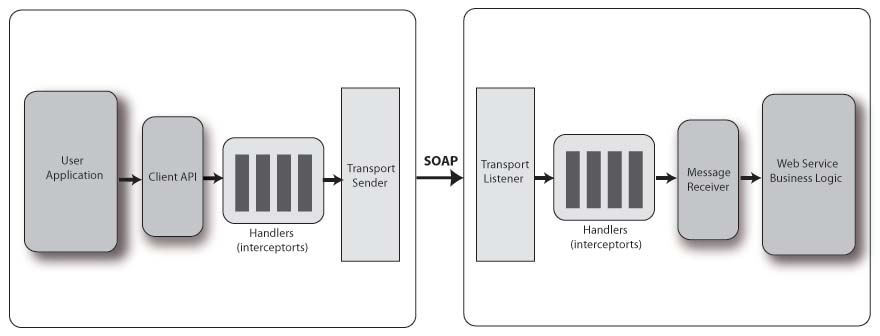
\includegraphics[scale=0.4]{img/obr1}};
\end{tikzpicture}
\begin{tikzpicture}[remember picture,overlay]
    \node[xshift=-0.6cm,yshift=-1.3cm] at (current page.north east){%
    
\includegraphics[width=0.8cm]{img/pozor}};
\end{tikzpicture}
\end{frame}


\begin{frame}[containsverbatim]\frametitle{JAX-WS Web Integration}
\begin{itemize}
	\item Glassfish Metro
	  \begin{itemize}
		\item Endpoint specified in \texttt{sun-jaxws.xml}
		\item \texttt{web.xml}
          \begin{itemize}
            \item \texttt{WSServletContextListener} --  listener class
            \item \texttt{WSServlet} -- web service servlet
          \end{itemize}
    	\item \texttt{@WebService}
		\item \texttt{@WebMethod}
      \end{itemize}
\end{itemize}
\end{frame}


\begin{frame}[containsverbatim]\frametitle{sun-jaxws.xml}
\begin{footnotesize}
          \begin{verbatim}
<?xml version="1.0" encoding="UTF-8"?>
<endpoints
  xmlns="http://java.sun.com/xml/ns/jax-ws/ri/runtime"
  version="2.0">
  <endpoint
    name="HelloWorldWs"
    implementation="cz.vutbr.fit.knot.gja.example.HelloWorld"
    url-pattern="/hello"/>
</endpoints>
\end{verbatim}
\end{footnotesize}
\end{frame}


\begin{frame}[containsverbatim]\frametitle{web.xml}
\begin{footnotesize}
          \begin{verbatim}
<web-app>
  <display-name>Archetype Created Web Application</display-name>
  <listener>
    <listener-class>
      com.sun.xml.ws.transport.http.servlet.WSServletContextListener
    </listener-class>
  </listener>
  <servlet>
    <servlet-name>hello</servlet-name>
    <servlet-class>
      com.sun.xml.ws.transport.http.servlet.WSServlet
    </servlet-class>
    <load-on-startup>1</load-on-startup>
  </servlet>
  <servlet-mapping>
    <servlet-name>hello</servlet-name>
    <url-pattern>/hello</url-pattern>
  </servlet-mapping>
</web-app>
\end{verbatim}
\end{footnotesize}
\begin{textblock}{5}(10.2,0.9)
    {\footnotesize Example JAX-WS-Web}
\end{textblock}
\end{frame}


\begin{frame}[containsverbatim]\frametitle{JAX-WS}
\begin{itemize}
  \item Endpoints
    \begin{itemize}
      \item RPC (Remote Procedure Call) style web service endpoint
      \item Document style web service endpoint
    \end{itemize}
\end{itemize}
\begin{tikzpicture}[remember picture,overlay]
    \node[xshift=-0.6cm,yshift=-1.3cm] at (current page.north east){%
    
\includegraphics[width=1cm]{img/pozor}};
\end{tikzpicture}
\begin{tikzpicture}[remember picture,overlay]
    \node[xshift=-0.6cm,yshift=-1.3cm] at (current page.north east){%
    
\includegraphics[width=1cm]{img/pozor}};
\end{tikzpicture}
\end{frame}


\begin{frame}[containsverbatim]\frametitle{JAX-WS RPC style}
\begin{itemize}
	\item Synchronous
	\item Easy to implement
	\item SOAP engine takes care of marshalling
	\item Poor performance
	\item Interface annotation
      \begin{itemize}
    	\item \texttt{@WebService}
		\item \texttt{@SOAPBinding(style = Style.RPC)}
      \end{itemize}
    \item Implementation
      \begin{itemize}
    	\item {\footnotesize \texttt{@WebService(endpointInterface = "package.Interface")}}
      \end{itemize}
    \item Accessible on URL commonly named by package
      \begin{itemize}
    	\item QName defines target service endpoint 
		\item Communication via service port
      \end{itemize}
\end{itemize}
\begin{tikzpicture}[remember picture,overlay]
    \node[xshift=-0.6cm,yshift=-1.3cm] at (current page.north east){%
    
\includegraphics[width=1cm]{img/pozor}};
\end{tikzpicture}
\end{frame}


\begin{frame}[containsverbatim]\frametitle{JAX-WS RPC example}
\begin{footnotesize}
\begin{verbatim}
// Service Endpoint Interface
@WebService
@SOAPBinding(style = Style.RPC)
public interface HelloWorld{
    @WebMethod String getHelloWorldAsString(String name);
}

// Service Implementation
@WebService(endpointInterface = "cz.vutbr.fit.knot.gja.ws.HelloWorld")
public class HelloWorldImpl implements HelloWorld{
    @Override
    public String getHelloWorldAsString(String name) {
        return "Hello World JAX-WS " + name;
    }
}

// Endpoint publisher
public class HelloWorldPublisher{
    public static void main(String[] args) {
        Endpoint.publish("http://localhost:9999/ws/hello", 
            new HelloWorldImpl());
    }
}
\end{verbatim}
\end{footnotesize}
\end{frame}


\begin{frame}[containsverbatim]\frametitle{JAX-WS RPC example (2)}
\begin{footnotesize}
\begin{itemize}
  \item It is possible to access deployed web service by accessing the generated WSDL (Web Service Definition Language) document via this URL \verb+http://localhost:9999/ws/hello?wsdl+
\end{itemize}
\begin{verbatim}
import javax.xml.namespace.QName;
import javax.xml.ws.Service;
...

public class HelloWorldClient {
  public static void main(String[] args) throws Exception {
    URL url = new URL("http://localhost:9999/ws/hello?wsdl");
    // 1st argument is service URI, refer to wsdl document above
    // 2nd argument is service name, refer to wsdl document above
    QName qname = new QName("http://ws.gja.knot.fit.vutbr.cz/", 
        "HelloWorldImplService");

    Service service = Service.create(url, qname);
    HelloWorld hello = service.getPort(HelloWorld.class);
    System.out.println(hello.getHelloWorldAsString("fit"));
  }
}
\end{verbatim}
\end{footnotesize}
\begin{tikzpicture}[remember picture,overlay]
    \node[xshift=-0.6cm,yshift=-1.3cm] at (current page.north east){%
    
\includegraphics[width=0.8cm]{img/oko}};
\end{tikzpicture}
\end{frame}


\begin{frame}[containsverbatim]\frametitle{JAX-WS RPC example (3)}
\begin{footnotesize}
\begin{itemize}
  \item Alternative, you can use \texttt{wsimport} tool to parse the published wsdl file, and generate necessary client files (stub) to access the published web service.
  \item[] \verb+wsimport -keep http://localhost:9999/ws/hello?wsdl+
\end{itemize}
\begin{verbatim}
import com.mkyong.ws.HelloWorld;
import com.mkyong.ws.HelloWorldImplService;

public class HelloWorldClient{
  public static void main(String[] args) {
    HelloWorldImplService helloService = new HelloWorldImplService();
    HelloWorld hello = helloService.getHelloWorldImplPort();

    System.out.println(hello.getHelloWorldAsString("fit"));
  }
}
\end{verbatim}
\end{footnotesize}
\begin{textblock}{5}(11.1,2.2)
    {\footnotesize Example JAX-WS}
\end{textblock}
\begin{tikzpicture}[remember picture,overlay]
    \node[xshift=-0.6cm,yshift=-1.3cm] at (current page.north east){%
    
\includegraphics[width=1cm]{img/oko}};
\end{tikzpicture}
\end{frame}


\begin{frame}[containsverbatim]\frametitle{JAX-WS Document style}
\begin{itemize}
	\item Used for implementing asynchronous service
	\item More time consuming to create
	\item Large size documents processed without significant performance drop
	\item Better custom data type definition
	\item Interface annotation
      \begin{itemize}
    	\item \texttt{@WebService}
		\item {\footnotesize \texttt{@SOAPBinding(style = Style.DOCUMENT, use=Use.LITERAL)}}
		\item \texttt{SOAPBinding.Use.ENCODED} -- SOAP message contains data type information
		\item \texttt{SOAPBinding.Use.LITERAL} -- SOAP message contains reference (namespace) to the schema that is used
      \end{itemize}
    
    \item Otherwise similar as RPC
\end{itemize}
\begin{tikzpicture}[remember picture,overlay]
    \node[xshift=-0.6cm,yshift=-1.3cm] at (current page.north east){%
    
\includegraphics[width=1cm]{img/pozor}};
\end{tikzpicture}
\end{frame}


\begin{frame}[containsverbatim]\frametitle{JAX-WS Document example}
\begin{footnotesize}
\begin{verbatim}
// Service Endpoint Interface
@WebService
@SOAPBinding(style = Style.DOCUMENT, use=Use.LITERAL) // optional
public interface HelloWorld {
  @WebMethod String getHelloWorldAsString(String name);
}

// Service Implementation
@WebService(endpointInterface = "cz.vutbr.fit.knot.gja.ws.HelloWorld")
public class HelloWorldImpl implements HelloWorld{
  @Override
  public String getHelloWorldAsString(String name) {
    return "Hello World JAX-WS " + name;
  }
}
// Endpoint publisher
public class HelloWorldPublisher{
  public static void main(String[] args) {
    Endpoint.publish("http://localhost:9999/ws/hello", 
      new HelloWorldImpl());
  }
}
\end{verbatim}
\end{footnotesize}
\end{frame}


\begin{frame}[containsverbatim]\frametitle{JAX-WS Document example (2)}
\begin{itemize}
  \item Document style requires extra classes to run. You need to use \texttt{wsgen} tool to generate necessary JAX-WS portable artifacts.
  \item[] \verb+wsgen -keep -cp . cz.vutbr.fit.knot.gja.ws.HelloWorld+
    \begin{itemize}
      \item It will generate two classes, copy it to your \texttt{package.jaxws} folder.
    \end{itemize}
  \item Publish it and test it via URL \verb+http://localhost:9999/ws/hello?wsdl+
\end{itemize}
\begin{tikzpicture}[remember picture,overlay]
    \node[xshift=-0.6cm,yshift=-1.3cm] at (current page.north east){%
    
\includegraphics[width=1cm]{img/oko}};
\end{tikzpicture}
\end{frame}


\begin{frame}[containsverbatim]\frametitle{JAX-WS Document example (3)}
\begin{footnotesize}
\begin{verbatim}
import javax.xml.namespace.QName;
import javax.xml.ws.Service;
...

public class HelloWorldClient{
  public static void main(String[] args) throws Exception {

    URL url = new URL("http://localhost:9999/ws/hello?wsdl");
    QName qname = new QName("http://ws.gja.knot.fit.vutbr.cz/",
                            "HelloWorldImplService");

    Service service = Service.create(url, qname);
    HelloWorld hello = service.getPort(HelloWorld.class);

    System.out.println(hello.getHelloWorldAsString("fit"));
  }
}
\end{verbatim}
\end{footnotesize}
\begin{textblock}{5}(9.1,1.6)
    {\footnotesize Example JAX-WS-Document}
\end{textblock}
\end{frame}


\begin{frame}[containsverbatim]\frametitle{JAX-WS MTOM}
\begin{itemize}
	\item Message Transmission Optimization Mechanism
	\item Sending binary attachments
	\item Combines Base64 with SOAP
	\item File upload
	\item File download
	\item MIME types
\end{itemize}
\begin{footnotesize}
\begin{verbatim}
// Service Implementation Bean
@MTOM
@WebService(endpointInterface = "cz.vut.fit.knot.gja.ws.ImageServer")
public class ImageServerImpl implements ImageServer{
  @Override
  public Image downloadImage(String name) {
...
\end{verbatim}
\begin{itemize}
  \item If the server WSDL advertises that it supports MTOM, the MTOM support in the client will be automatically enabled.
\end{itemize}
\end{footnotesize}
\begin{textblock}{5}(9.9,0.9)
    {\footnotesize Example JAX-WS-MTOM}
\end{textblock}
\begin{tikzpicture}[remember picture,overlay]
    \node[xshift=-0.6cm,yshift=-1.3cm] at (current page.north east){%
    
\includegraphics[width=1cm]{img/pozor}};
\end{tikzpicture}
\end{frame}


\begin{frame}[containsverbatim]\frametitle{JAX-WS architecture}
\begin{tikzpicture}[remember picture,overlay]
    \node[xshift=-6.4cm,yshift=-5.5cm] at (current page.north east) {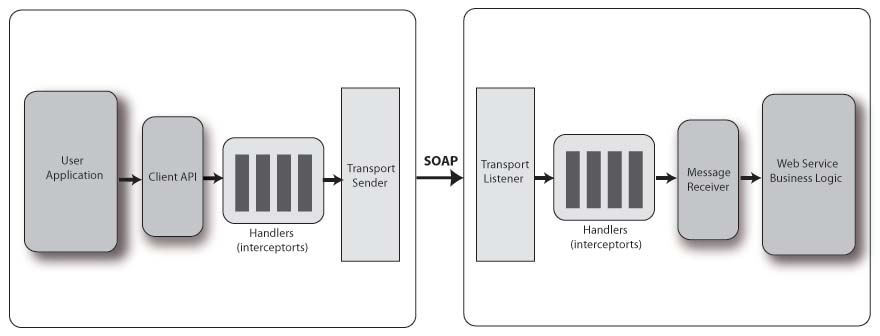
\includegraphics[scale=0.4]{img/obr1}};
\end{tikzpicture}
\end{frame}

\begin{frame}[containsverbatim]\frametitle{Web Service handlers}
\begin{itemize}
	\item Client handlers
	  \begin{itemize}
		\item intercept client calls to server
		\item injects authentication
		\item adds MAC, IP address, \ldots
	  \end{itemize}
    \item Server interceptors
	  \begin{itemize}
		\item retrieves information from SOAP header block
		\item authorizes client
	  \end{itemize}
\end{itemize}
\begin{tikzpicture}[remember picture,overlay]
    \node[xshift=-0.6cm,yshift=-1.3cm] at (current page.north east){%
    
\includegraphics[width=1cm]{img/oko}};
\end{tikzpicture}
\end{frame}

\begin{frame}[containsverbatim]\frametitle{Client handler}
\begin{itemize}
	\item Create the client for the web service
	\item Create SOAP Handler
	\item Handler Configuration
	\item Handler Mapping Tracing the outgoing and incoming messages in success and failure case
	\item SOAPHandler interface
    \item[] \begin{footnotesize}\begin{verbatim}
public class MySOAPHandler 
    implements SOAPHandler<SOAPMessageContext> {
  @Override
  public boolean handleMessage(SOAPMessageContext 
      messagecontext) {
    Boolean outbound = (Boolean) messagecontext.get(
      MessageContext.MESSAGE_OUTBOUND_PROPERTY);
    ...
    SOAPMessage message = messagecontext.getMessage();
    SOAPHeader header = message.getSOAPHeader();
    SOAPBody body = message.getSOAPBody();
    ...
\end{verbatim}
\end{footnotesize}
  \item handleMessage returns true to continue processing, false to block processing.
\end{itemize}
\begin{tikzpicture}[remember picture,overlay]
    \node[xshift=-0.6cm,yshift=-1.3cm] at (current page.north east){%
    
\includegraphics[width=1cm]{img/oko}};
\end{tikzpicture}
\end{frame}


\begin{frame}[containsverbatim]\frametitle{Client handler (2)}
\begin{itemize}
    \item Interceptor mapping specified in XML file	
    \begin{itemize}
    	\item \texttt{@HandlerChain}
		\item More mapping possible
        \item[] \begin{footnotesize}
      \begin{verbatim}
@WebServiceClient(name = "ServerInfoService",
  targetNamespace = "http://ws.gja.knot.fit.vutbr.cz/",
  wsdlLocation = "http://localhost:8888/ws/server?wsdl")
@HandlerChain(file="handler-client.xml")
public class ServerInfoService extends Service
{
  // ...
}
      
<?xml version="1.0" encoding="UTF-8" standalone="yes"?>
<jakartaee:handler-chains
    xmlns:jakartaee="https://jakarta.ee/xml/ns/jakartaee"
    xmlns:xsd="http://www.w3.org/2001/XMLSchema">
  <jakartaee:handler-chain>
    <jakartaee:handler>
      <jakartaee:handler-class>
      cz.vutbr.fit.knot.gja.ws.client.MacAddressInjectHandler
      </jakartaee:handler-class>
    </jakartaee:handler>
  </jakartaee:handler-chain>
</jakartaee:handler-chains>
\end{verbatim}
    \end{footnotesize}
    \end{itemize}   
\end{itemize}
\end{frame}


\begin{frame}[containsverbatim]\frametitle{Server handler}
\begin{itemize}
	\item Create Web Service
	\item Create SOAP Handler
	\item Handler Configuration
	\item Handler Mapping
	\item SOAPHandler interface
      \begin{itemize}
    	\item \texttt{SOAPMessageContext}
		\item \texttt{handleMessage} returns true or false (chain may be broken)
      \end{itemize}
\end{itemize}
\end{frame}

\begin{frame}[containsverbatim]\frametitle{Server handler (2)}
\begin{itemize}
    \item Intercept mapping specified in XML file	
      \begin{itemize}
    	\item \texttt{@HandlerChain}
		\item More mapping possible
        \item[] \begin{footnotesize}
      \begin{verbatim}
@WebService
@HandlerChain(file="handler-server.xml")
public class Server{
  @WebMethod
  public String getServerName() {
    return "localhost server";
  }
}

<?xml version="1.0" encoding="UTF-8" standalone="yes"?>
<jakartaee:handler-chains
    xmlns:jakartaee="https://jakarta.ee/xml/ns/jakartaee"
    xmlns:xsd="http://www.w3.org/2001/XMLSchema">
  <jakartaee:handler-chain>
    <jakartaee:handler>
      <jakartaee:handler-class>
   cz.vutbr.fit.knot.gja.ws.server.MacAddressValidatorHandler
      </jakartaee:handler-class>
    </jakartaee:handler>
  </jakartaee:handler-chain>
</jakartaee:handler-chains>
\end{verbatim}
      \end{footnotesize}
      \end{itemize}   
\end{itemize}
\begin{textblock}{5}(9.7,-0.3)
    {\footnotesize Example JAX-WS-Handler}
\end{textblock}
\end{frame}


\begin{frame}[containsverbatim]\frametitle{References}
\begin{itemize}
	\item JAX-WS
      \begin{itemize}
    	\item \url{http://www.mkyong.com/tutorials/jax-ws-tutorials/}
        \item \url{https://www.mkyong.com/webservices/jax-ws/jax-ws-java-web-application-integration-example/}
        \item \url{https://www.mkyong.com/webservices/jax-ws/jax-ws-soap-handler-in-client-side/}
        \item \url{https://www.mkyong.com/webservices/jax-ws/jax-ws-soap-handler-in-server-side/}
        \item \url{https://web.archive.org/web/20211023024040/http://blog.jdevelop.eu/?p=67}
        \item \url{https://metro.java.net/nonav/1.2/docs/}
        \item \url{https://docs.oracle.com/javaee/7/api/}
        \item \url{https://jcp.org/en/jsr/detail?id=224}
        \item \url{http://javainsimpleway.com/jax-ws-basic-example-document-style/}
      \end{itemize}
    \item SOAP
      \begin{itemize}
    	\item \url{https://www.w3.org/TR/soap12-part0/}
        \item \url{https://www.w3schools.com/xml/xml_soap.asp}
        \item \url{https://www.ibm.com/support/knowledgecenter/en/SSB27H_6.2.0/fa2ws_ovw_soap_syntax_lit.html}
      \end{itemize}
\end{itemize}
\end{frame}


\bluepage{Thank you for your attention!}


\end{document}
